\chapter{Preliminaries}\label{preliminaries}

In this Chapter, the models, algorithms and objectives of the two basic word embedding algorithms Word2vec and Doc2vec are described.

\section{Word2vec}

The term Word2vec summarizes two different models: the distributed bag of words model (CBOW) and the continuous skip-gram model (skip-gram). Both use neural networks, and they work very similarly. However, they have very different objectives and thus are able to capture different syntactic and semantic patterns. Furthermore, they both have different parameters. Let us have a closer look.

\subsection{Objectives}

In the paper, two different objectives for the CBOW model are proposed. Mathematically, this can be expressed in two formulas, where $w_{j}$ is the $j$-th word, and $c$ is the window size. The first objective is to predict the next word-based on $c$ previously encountered words.
\begin{displaymath}
  \underset{W}{\text{maximize}}\ p(w_{t} | w_{t - c},\ w_{t - (c-1)},\ \ldots,\ w_{t - 2},\ w_{t - 1})
\end{displaymath}
The second objective is to predict the word in the middle of $c$ previously encountered words and $c$ following words.
\begin{displaymath}
  \underset{W}{\text{maximize}}\ p(w_{t} | w_{t - c},\ w_{t - (c-1)},\ \ldots,\ w_{t - 1},\ w_{t + 1},\ \ldots,\ w_{t + (c-1)},\ w_{t + c})
\end{displaymath}
In this thesis, CBOW will always use the second objective, which is predicting the middle word from surrounding words. This leads to the objective of maximizing the average log probability.
\begin{displaymath}
 \underset{W}{\text{maximize}}\ \frac{1}{T} \sum_{t=1}^{T}\ \sum_{-c \leq j \leq c, j \neg 0} \log p(w_{t}|w_{t + j})
\end{displaymath}

While the CBOW model tries to predict the middle word given a context, the skip-gram model tries to do the opposite, which is to predict the surrounding words given a single word.
\begin{displaymath}
  \underset{W}{\text{maximize}}\ p(w_{t - c},\ w_{t - (c-1)},\ \ldots,\ w_{t - 1},\ w_{t + 1},\ \ldots,\ w_{t + (c-1)},\ w_{t + c} | w_{t})
\end{displaymath}
Again, this leads to the objective of maximizing the average log probability.
\begin{displaymath}
 \underset{W}{\text{maximize}}\ \frac{1}{T} \sum_{t=1}^{T}\ \sum_{-c \leq j \leq c, j \neg 0} \log p(w_{t + j}|w_{t})
\end{displaymath}

\subsection{Neural Network Language Model}

To achieve the objectives described above, one recurrent neural network per objective is used. In the next few paragraphs, the neural network for the CBOW model is described. The neural network for the skip-gram model works analogous. The differences to the CBOW model are described at the end of this subsection.

The neural network consists of four layers: one input layer $I$, one projection layer $P$, one hidden layer $H$, and one output layer $V$. To model the weights of the connections between each connected layer, we use matrices. Since each two connected layers are fully connected to each other, the dimensionality of these matrices is the dimensionality of the upper layer times the dimensionality of the lower layer.

\begin{figure}
	\centering
	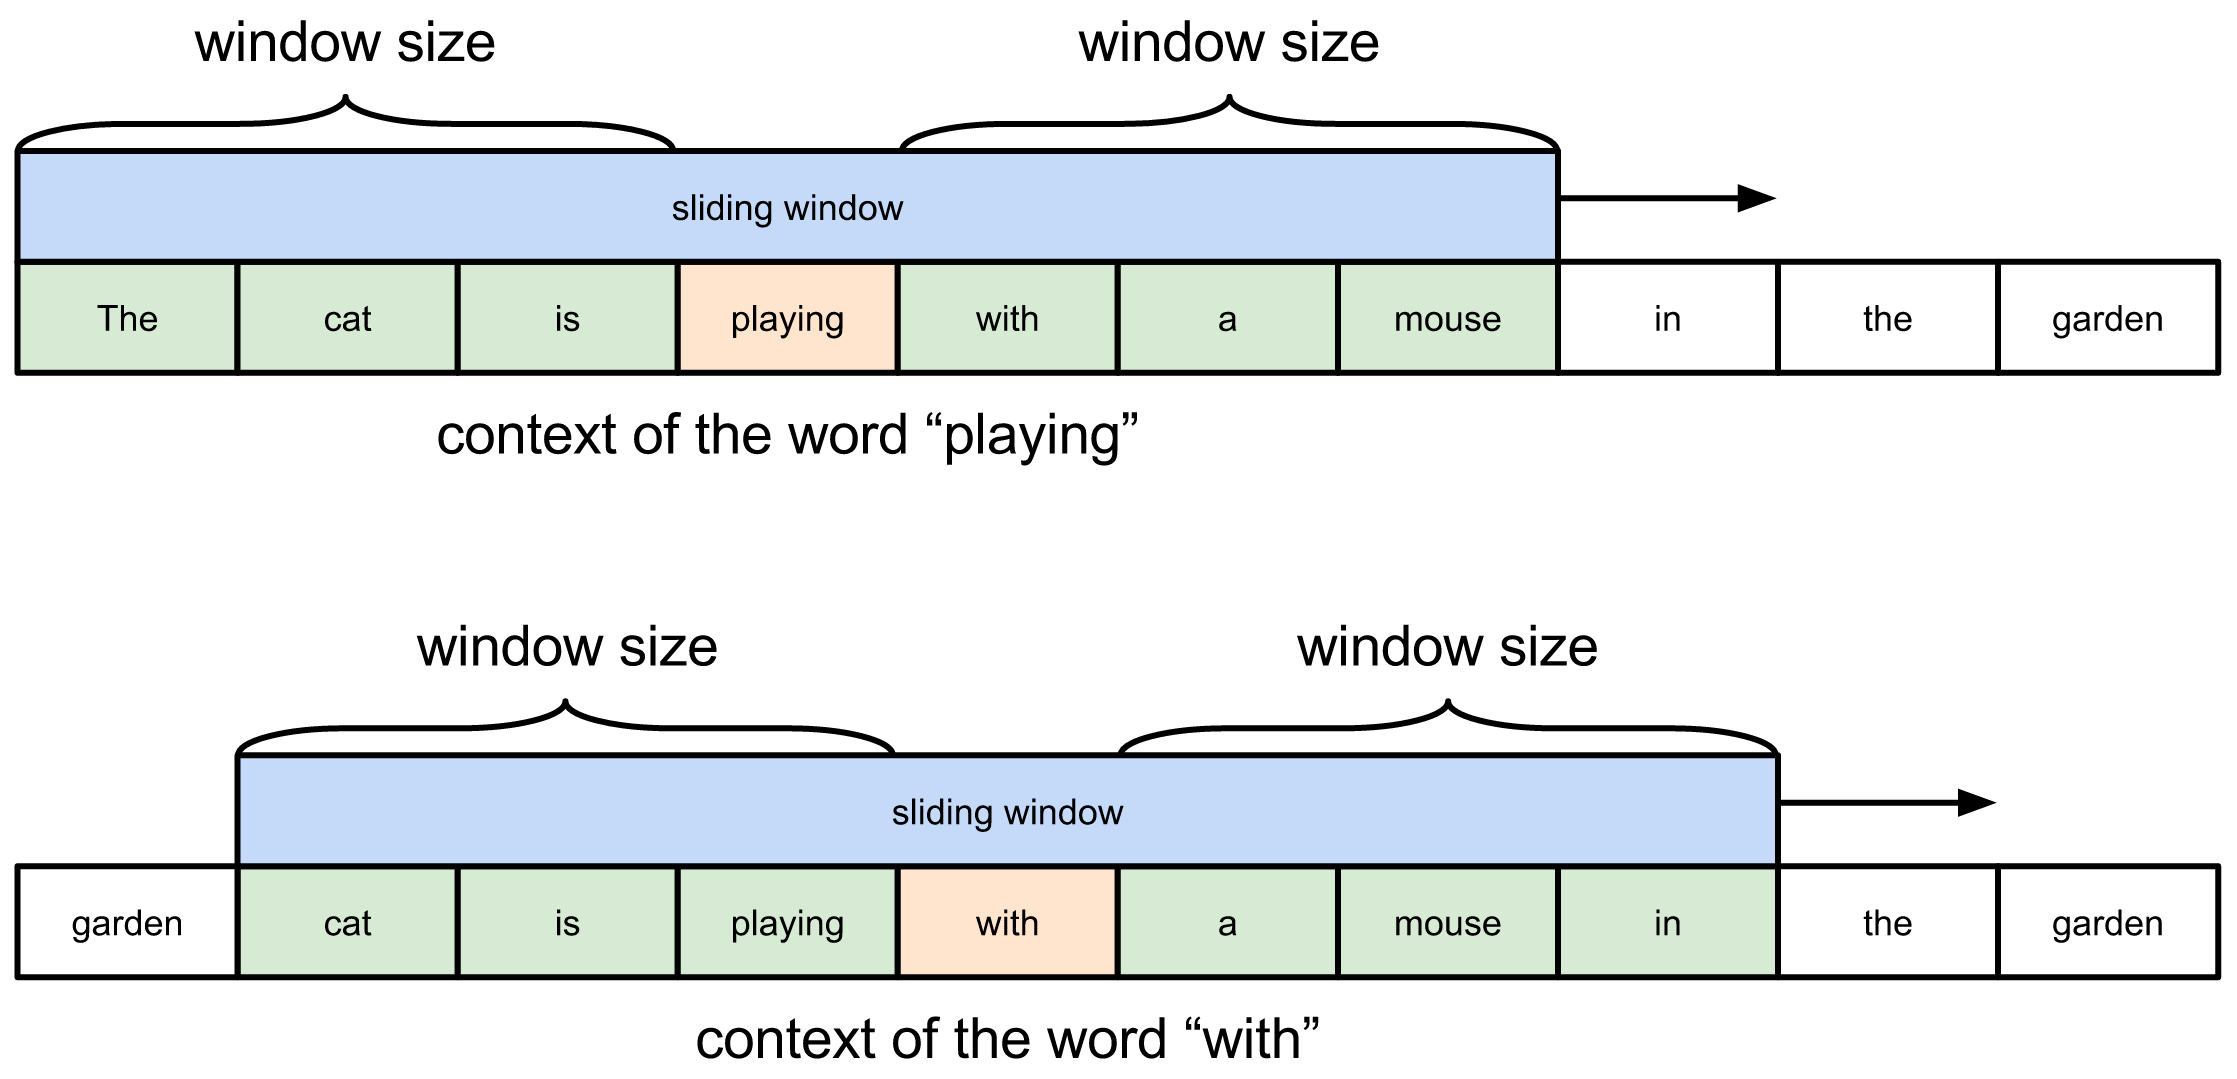
\includegraphics[width=0.9\textwidth]{3preliminaries/sliding-window}
	\caption{The window size of the sliding window defines which words are in the context of the middle word.}
	\label{fig:3:sliding-window}
\end{figure}

In the input layer, all words in the context of a word are listed, while the context is defined by the window size $c$. For example, if $c=3$, then the context for the word ``playing'' of the sentence ``The cat is \emph{playing} with a mouse in the garden'' is [the, cat, is, with, a, mouse], and the context for the word ``with'' is [cat, is, playing, a, mouse, in], see Figure~\ref{fig:3:sliding-window}. Therefore, the dimensionality of $I$ is two times the window size $c$.
\begin{displaymath}
\dim(I) = 2c
\end{displaymath}

Next, every word in the context is mapped to a $d$ dimensional vector, where $d$ is the word vector dimensionality. The weights of this projection define the resulting word vector. The dimensionality of the projection layer is the dimensionality of the input layer times the word vector dimensionality.
\begin{displaymath}
\dim(P) = \dim(I) \times d = 2c \times d
\end{displaymath}

An equivalent model of the input and projection layer is to use the whole vocabulary $U$ as input layer, while the words in the context are encoded with a 1 and the ones not in the context with a 0. Then the projection layer consists of all word vectors, and thus does not have to be changed when the context words change. Since the words that are not in the context are encoded as 0, the corresponding word vectors are multiplied by 0 and thus do not contribute to the prediction.

The hidden layer is fully connected to the projection layer, and has arbitrary dimensionality, usually between 500 and 2000.
\begin{displaymath}
\dim(H) = x \in [500,\ 2000]
\end{displaymath}

Finally, the output layer has the same dimensionality as $U$, where the $j$-th value $v_{j}$ is a score to calculate the conditional probability that the $j$-th word $w_{j}$ occurs given the context $w_{x - c},\ \ldots\ ,w_{x + c}$. In the next subsection, we describe how to calculate these conditional probabilities.
\begin{displaymath}
\dim(V) = \dim(U)
\end{displaymath}

Now let us consider the skip-gram model. The input layer consists of only one word, and the projection and the hidden layer have the same architecture and meaning as in the CBOW model. However, instead of having only one multinomial distribution, we have $2c$ multinomial distributions, one for each word in the context. Thus, the dimensionality of the neural network for CBOW is different.
\begin{displaymath}
\begin{aligned}
\dim(I) &= 1 \\
\dim(P) &= d \\
\dim(H) &= x \in [500,\ 2000] \\
\dim(V) &= 2c \times \dim(U)
\end{aligned}
\end{displaymath}

\subsection{Algorithm}

As in the common neural network, the weights are learned via gradient descent and backpropagation. Let us again consider the algorithm for the CBOW\@. First, each word vector (one per word) is initialized randomly. Next, the documents are processed using a sliding window of size $c$ (usually between 5 and 20). Then, the word vectors of the context are set as the projection layer, and the network tries to predict the middle word. The error gradient is then calculated and backpropagated by using soft-max. $v_j$ is the value in the output layer per word in the vocabulary $U$.
\begin{displaymath}
p(w_{t} | w_{t - c},\ \ldots,\ w_{t + c}) = \frac{e^{v_{j}}}{\sum_{j'=1}^{\dim(U)}\ e^{v_{j'}}}
\end{displaymath}

This conditional probability is then compared to the actual output (the middle word). Based on the result (overestimation or underestimation), the error is backpropagated through the neural network, and the weights for the word vectors in this context are updated accordingly.

For example, consider again the sentence ``The cat is playing with a \emph{mouse} in the garden'' with a window size $c=3$ and the word to predict being ``mouse''. If the network predicts that the word ``cat'' is probable to appear (however, ``cat'' does not appear in the context of ``mouse''), then this error is backpropagated and the word vectors for [playing, with, a, in, the, garden] are updated. In contrast, if the word ``mouse'' is predicted to be appearing in this context, the error is small and thus the backpropagation will not change the vectors [playing, with, a, in, the, garden] significantly.

The skip-gram algorithm works analogously to the CBOW model. It tries to predict the context of $w_{j}$, and backpropagates the mean error to change the word vector of $w_{j}$ accordingly.

\begin{figure}
	\centering
	\begin{subfigure}{.5\textwidth}
		\centering
		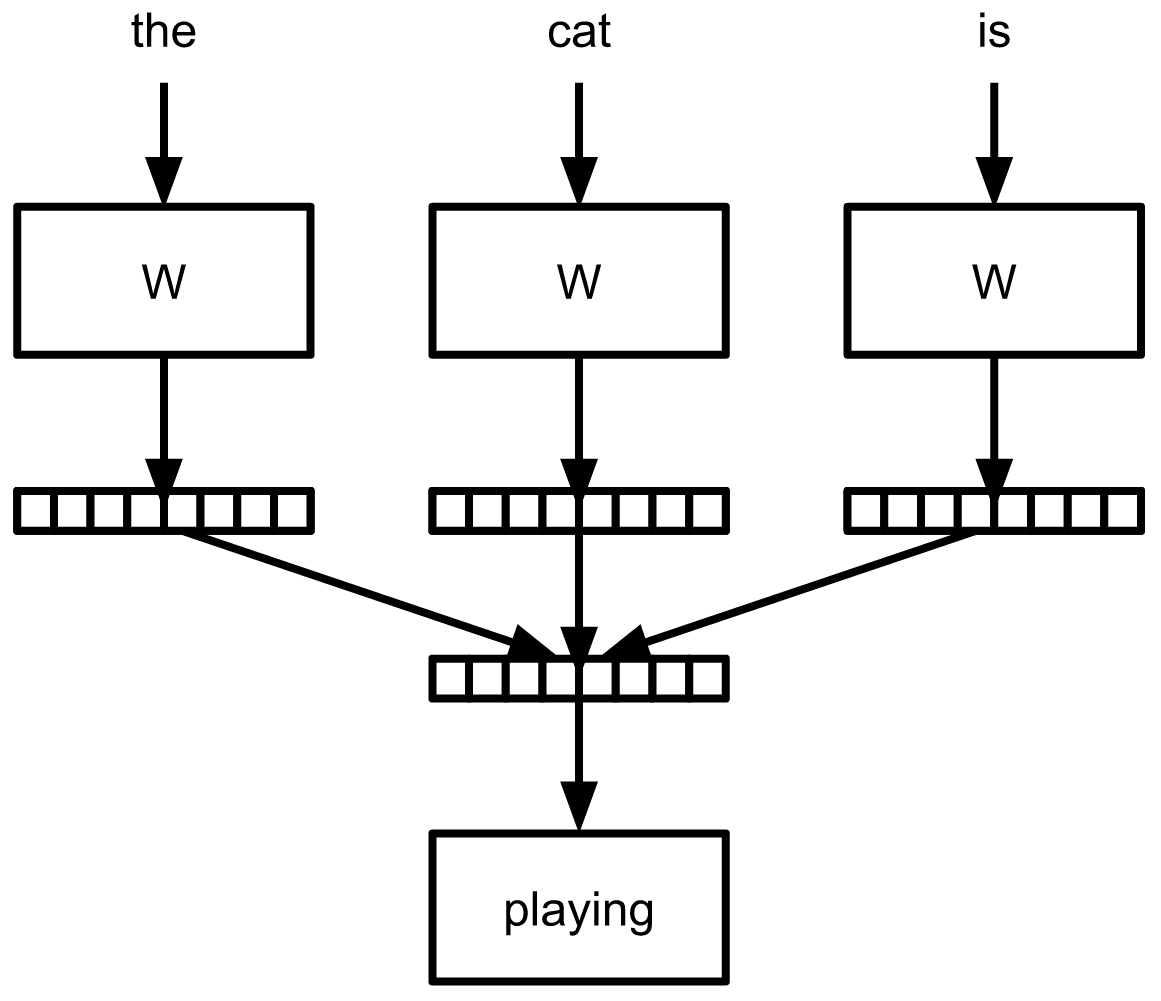
\includegraphics[width=1.0\linewidth]{3preliminaries/cbow}
		\caption{CBOW}
		\label{fig:3:cbow}
	\end{subfigure}\begin{subfigure}{.5\textwidth}
		\centering
		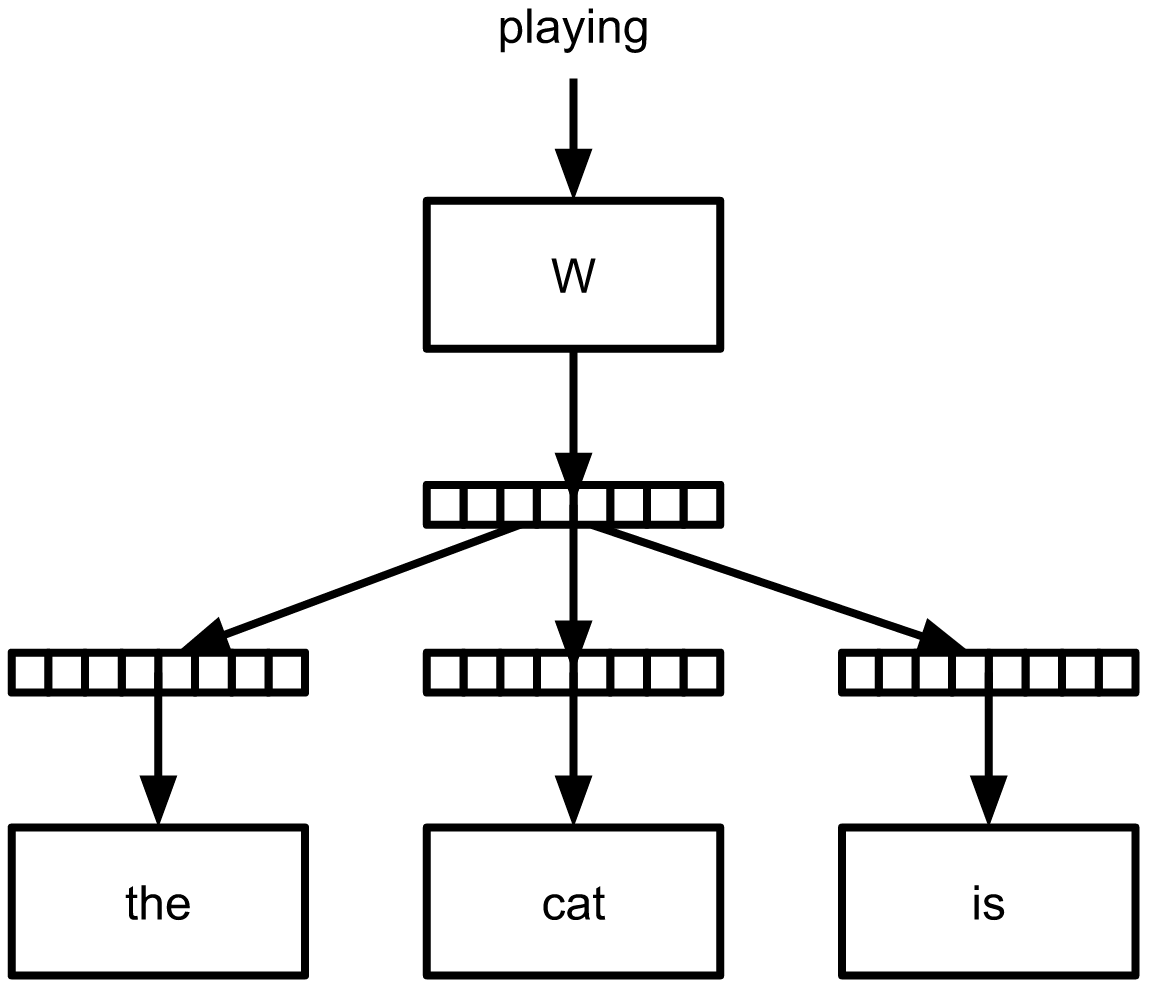
\includegraphics[width=1.0\linewidth]{3preliminaries/sg}
		\caption{Skip-gram}
		\label{fig:3:sg}
	\end{subfigure}
	\caption{The architecture of the neural network for CBOW and skip-gram. On the top is the input layer, in the middle the hidden layer, and in the bottom the output layer.}
	\label{fig:3:cbow-sg}
\end{figure}

The two architectures are sketched in Figure~\ref{fig:3:cbow-sg}. For a more extensive description on how exactly the Word2vec parameters are learned, see~\cite{Mikolov2013a, Mikolov2013, TomasMikolov, Rong2014, Goldberg2014a}.

\subsection{Computational Optimizations}

%resolved repetition:  Furthermore, the ultimate generalization is to train on an infinite amount of data, and thus being able to process a vast amount of text in a short time is a huge advantage.
While the two models CBOW and skip-gram discussed above are useful for understanding the basic models, these algorithms are computationally very inefficient. This is especially true when the vocabulary is large. Since there are nearly infinite amounts of written text available (for example Wikipedia, books, news, blogs) to train word embeddings on, it is imperative to minimize computational complexity in order to maximize accuracy by processing more text in less time. In this subsection, we will briefly describe the theoretical optimizations. As we will later see in Chapter~\ref{experiments}, additional optimizations regarding the implementation are also key to good results.

Since these optimizations are not necessary for understanding this thesis, we will only very briefly describe each concept. Interested readers can refer to~\cite{Mikolov2013, Rong2014, Goldberg2014a} to understand these optimizations in greater depth.

\emph{Hierarchical soft-max}~\cite{Morin2005, Mnih2009} calculates an approximated soft-max more efficiently.

\emph{Negative sampling}~\cite{Mikolov2013, Goldberg2014a} is a replacement for the soft-max and samples for every word $w_{j}$ $n$ words (usually between 5 and 20) from the vocabulary which are assumed not to appear with $w_{j}$.

Finally, \emph{sub-sampling of frequent words}~\cite{Mikolov2013} favors rare words compared to frequent words, as rare words are more probable to contribute important information compared to frequent words like stop words. This is similar to the IDF part of TF-IDF\@.

\section{Doc2vec}

As described in the previous section, Word2vec works with a sliding window of a fixed size. Again, let us consider the sentence ``The cat is playing with a mouse in the garden.''. If $c=3$, the words ``cat'' and ``garden'' will never occur together, and thus their respective word vectors will not be close to each other.

Doc2vec changes exactly that by adding an additional paragraph vector to each ``paragraph''. But let us first describe what is meant by a paragraph: a ``paragraph'' is a text block with arbitrary length, for example a chapter, a section, a text paragraph or a sentence. In this section, the word ``paragraph'' should describe such a text block of arbitrary length, and a paragraph vector (PV) is a vector for such a paragraph, like a word vector is to a word.

Let us continue with the paragraph vector characterization. This paragraph vector serves as a common context, which is shared within the paragraph. In the previous example ``The cat is playing with a mouse in the garden.'', the paragraph vector allows to share a context between ``cat'' and ``garden''. This vector can also be thought of as a word which appears in the context of a larger entity than the sliding window size allows.

One key advantage of Doc2vec is that it can easily be built into Word2vec. Essentially, each paragraph vector is a word vector which appears in every context of the current paragraph. It can be trained the same way as the word vectors through gradient descent and backpropagation, using the same neural network.

The PV enhanced CBOW model is called paragraph vector distributed memory (PV-DM) to stress the role of the PV to act as distributed memory. For the skip-gram model, the PV enhanced model is called PV-DBOW and is illustrated in Figure~\ref{fig:3:pv-dbow-pv-dm}.

\begin{figure}
	\centering
	\begin{subfigure}{.575\textwidth}
		\centering
		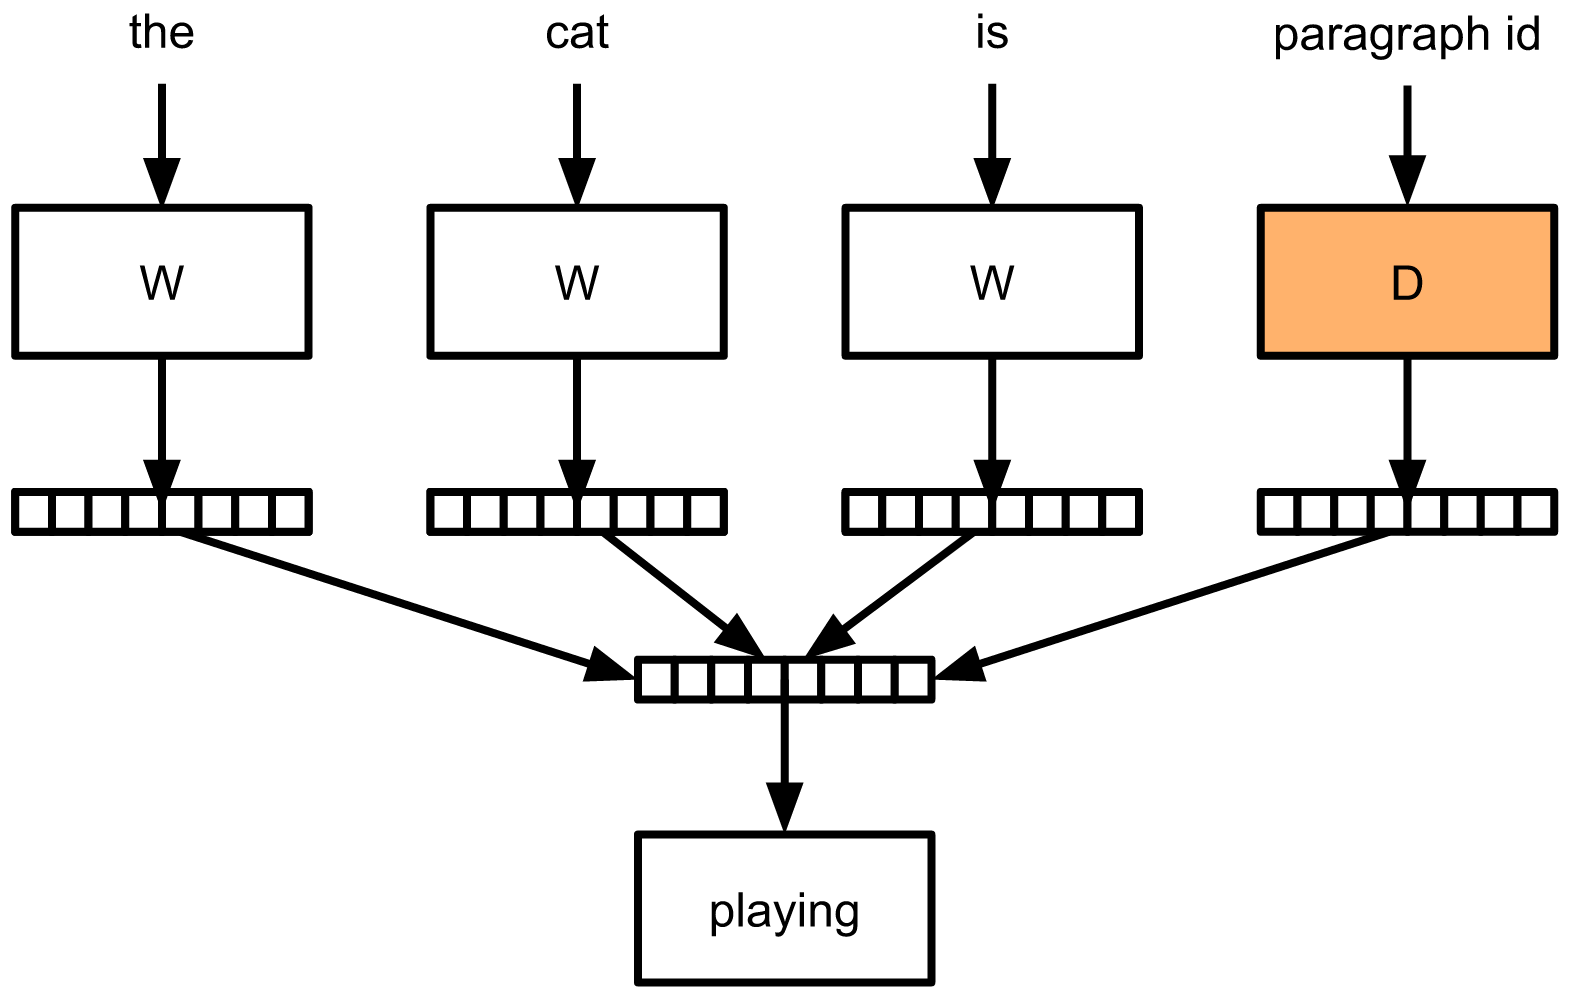
\includegraphics[width=1.0\linewidth]{3preliminaries/pv-dm}
		\caption{PV-DM}
		\label{fig:3:pv-dm}
	\end{subfigure}\begin{subfigure}{.425\textwidth}
	\centering
	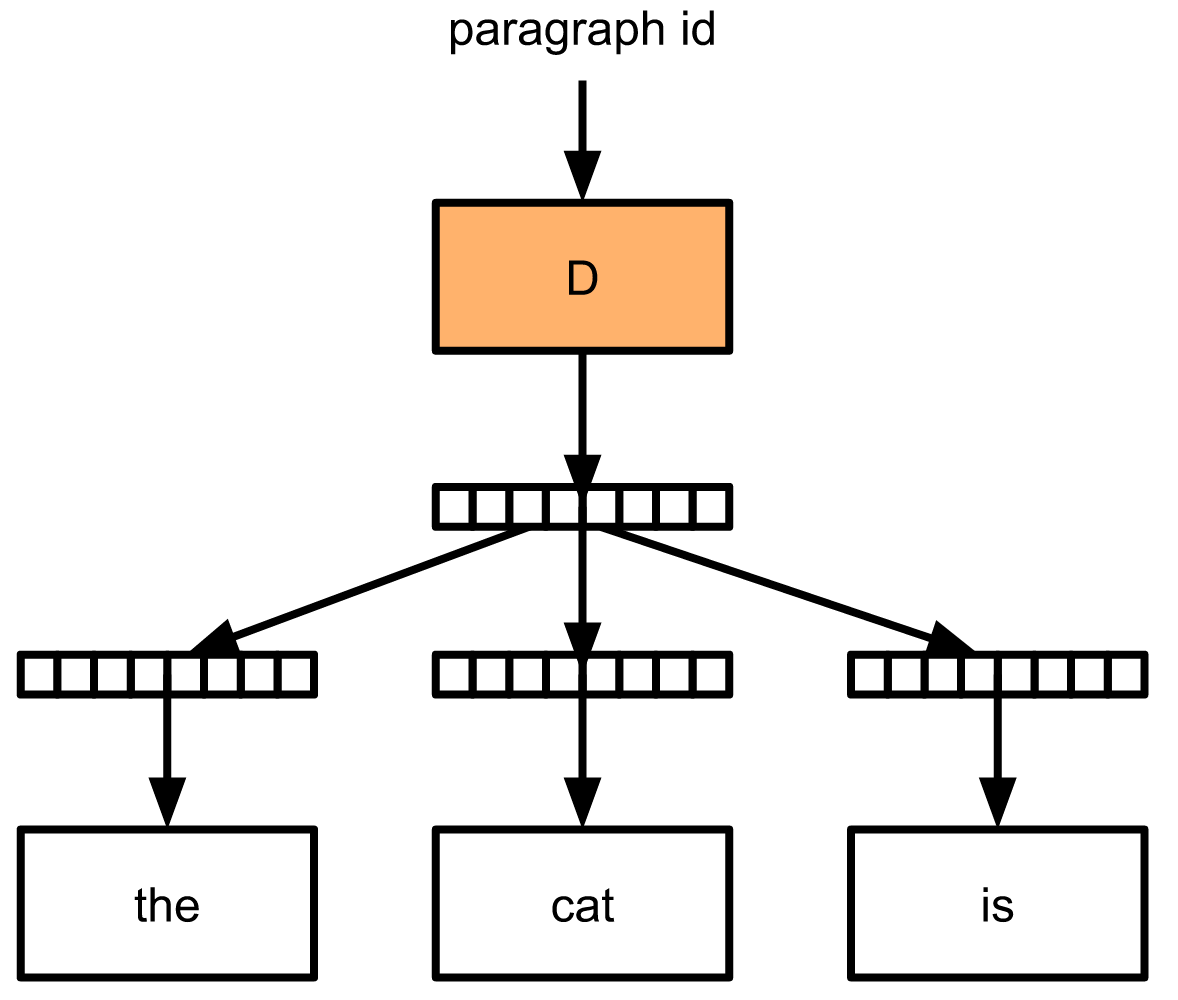
\includegraphics[width=1.0\linewidth]{3preliminaries/pv-dbow}
	\caption{PV-DBOW}
	\label{fig:3:pv-dbow}
	\end{subfigure}
\caption{The architecture of the neural network for PV-DM and PV-DBOW\@. On top is the input layer, in the middle the hidden layer, and in the bottom the output layer.}
\label{fig:3:pv-dbow-pv-dm}
\end{figure}
